\chapter{Dimensionering}

Figur \ref{fig:hej} viser de nye byggefelter inden for henholdsvis delområde A og delområde B til Strøybergs Palæ (\citep{lokalplan}, s. 16). Denne rapport fokuserer på byggefeltet inden for delområde B, hvor ny bebyggelse, ifølge lokalplan 1-1-107, må opføres i 3 etager samt en tagetage og med en kælder maksimalt 2 m over terræn. Ved opførsel af ny bebyggelse i delområde B, skal to nuværende mindre bygninger fjernes. 

\begin{figure}[htbp]
	\centering
	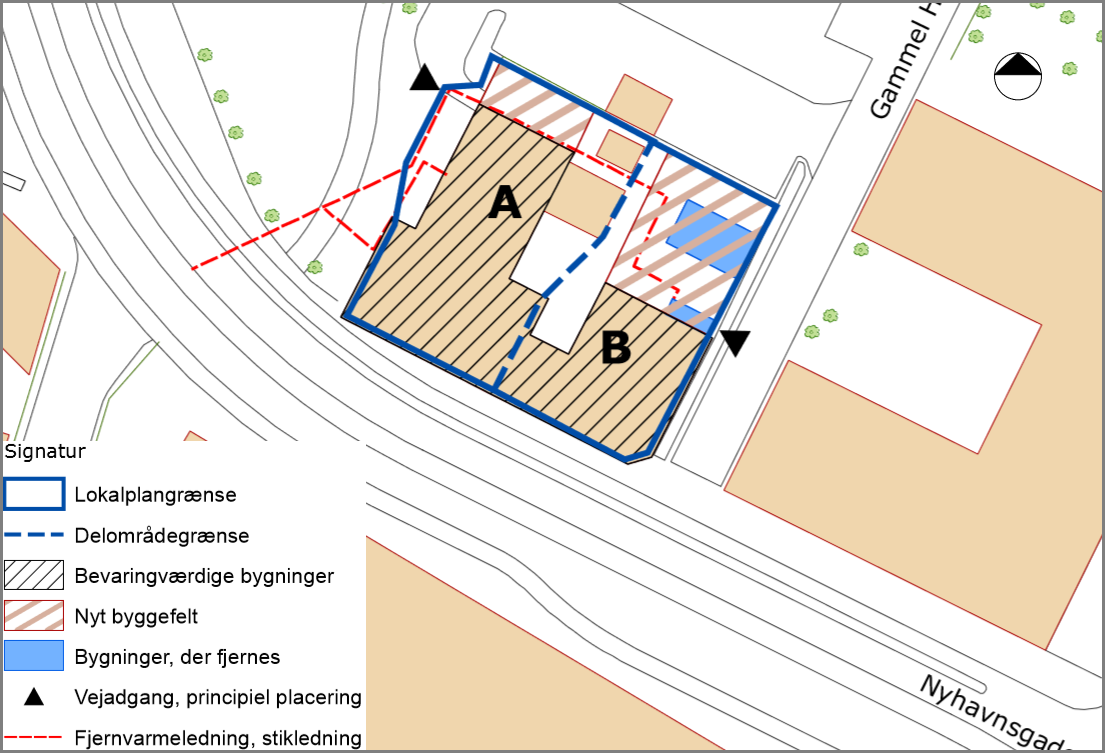
\includegraphics[width=0.7\textwidth]{billeder/signatur.png}
	\caption{Lokalplan 1-1-107, delområde A og B}
	\label{fig:hej}
\end{figure}

Med udgangspunkt i lokalplan 1-1-107 har bygningen fået de størrelser og dimensioner, som ses på Figur \ref{fig:farvel}.
\newline \indent{     }  Tilbygningen bliver 12,5 meter lang og 12 meter bred i henhold til den eksisterende bygningsbredde. Kælderen har en højde på i alt 3,25 m, hvor 1,25 m ligger over terræn. Stueetagen, 1. sal og 2. sal har hver især en højde på 4,9 m og tagetagen har en højde på 3 meter med en hældning på 26,6 grader. I alt er tilbygningen 19 m høj over terræn.

\begin{figure}[htbp]
	\centering
	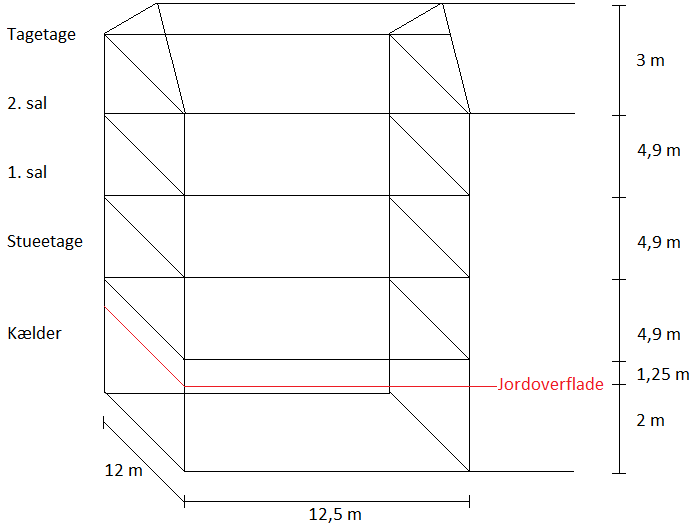
\includegraphics[width=0.7\textwidth]{billeder/tilbygning2.png}
	\caption{Tilbygningens dimensioner}
	\label{fig:farvel}
\end{figure}
/newline
For at kunne beregne de laster som påvirker tilbygningen, er der opstillet nedenstående statisk system for bygningen. Systemet er opstillet som en bjælkekonstruktion.

\section{Laster}
Lidt tekst her.

\subsection{Permanent last}
Indsætte her.

\subsection{Variable laster}
Af variable laster optræder der både snelast og vindlast på bygningen, og disse udregnes efter Dansk Standard Eurocode 1991.

\subsubsection{Snelast}
Indsætte her.

\subsubsection{Vindlast}
Vindlasten beregnes for det højeste punkt på konstruktionen, hvilket er på tagspidsen for tilbygningen, da det er det punkt, hvor vinden er kraftigst.
\newline
\newline
FIGUR!
\newline
\newline
Til at bestemme vindlasten på tilbygningen bruges følgende formel:	
\begin{center} $w_e=q_p(z_e)$$\cdot$$c_{pe}$}
\end{center}
$q_p$: peakhastighedstrykket
\newline
$z_e$: referencehøjden for det udvendige vindtryk
\newline
$c_{pe}$: formfaktoren for det udvendige vindtryk 
\newline
\newline
Den maksimale belastning fra vinden, peakhastighedstrykket $q_p$, bestemmes ved:
\begin{center}
$q_p(z_e)=[1+7I_v(z_e)]$$\cdot$$\frac{1}{2}$$\cdot$p$\cdot$$v_m^2(z_e)$
\end{center}
$I_v$: vindturbulens
\newline
$v_m$: middelvindhastigheden
\newline
\newline
For at bestemme peakhastigheden, beregnes først vindturbulens $I_v(z)$ samt middelvindhastigheden $v_m$.
\newline
\newline
Vindturbulens, $I_v(z)$, bestemmes ved:
\begin{center}
$I_v(z)=\frac{\sigma_v}{V_m(z)}=\frac{k_1}{c_0(z)\cdot ln(\frac{z}{z_0})}$
\end{center}
$k_1$: turbulensfaktor, sættes til 1.0 (\citep{EU91}, s. 82)
\newline
$c_0(z)$: orografifaktoren, som sættes til 1.0 (\citep{EU91}, s. 78)
\newline
$z$: højde, som er 19 m
\newline
$z_0$: ruhedslængde, som sættes til 1.0 for terrænkategori IV (\citep{EU91}, s.79)
\newline
\newline
Middelvindhastigheden, $v_m$, bestemmes ved:
\begin{center}
$v_m(z)=c_r(z)\cdot c_0(z)\cdot v_b$
\end{center}
$c_r(z)$: ruhedsfaktor
\newline
$v_b$: basisvindhastigheden
\newline
\newline
Til at bestemme middelvindhastigheden, beregnes basisvindhastigheden samt ruhedsfaktor.
\newline
\newline
Basisvindhastigheden, $v_b$, bestemmes ved:
\begin{center}
$v_b=c_{dir}\cdot c_{season}\cdot v_{b,0}$
\end{center}
$c_{dir}$: retningsfaktor, som sættes til 1.0 (\citep{EU91}, tabel 1a s. 77)
\newline
$c_{season}$: årstidsfaktor, som sættes til 1.0 (\citep{EU91}, tabel 1b s. 77)
\newline
$v_{b,0}$: grundværdi for basisvindhastigheden, som sættes til 24 $\frac{m}{s}$, da dette er gældende for størstedelen af Danmark (\citep{EU91}, s. 77)
\newline
\newline
Ruhedsfaktor, $c_r(z)$, bestemmes ved:
\begin{center}
$c_r(z)=k_r\cdot ln(\frac{z}{z_0})$
\end{center}
$k_r$: terrænfaktor
\newline
\newline
Terrænfaktoren, $k_r$, bestemmes ved:
\begin{center}
$k_r=0.19\cdot (\frac{z_0}{z_{0,II}})^{0.07}$
\end{center}
$z_{0,II}$: værdi for ruhedslængde for terrænkategori II, som sættes til 0.05 (\citep{EU91}, s. 78-79)

